\documentclass[a4paper,12pt]{article}
\usepackage[margin=0.7in]{geometry}
\usepackage[latin1]{inputenc}
\usepackage[english]{babel}
\usepackage{amsmath}
\usepackage{cases}
\usepackage[makeroom]{cancel}
\usepackage{amsmath,tabu}
\usepackage[fleqn]{mathtools}
\usepackage[fleqn]{amsmath}
\usepackage{bm}
\usepackage{tikz}
\usepackage{enumitem}
\usepackage{wrapfig}
\usepackage{graphicx}
\usepackage{siunitx}
\usepackage{microtype}
\usepackage{array,tabularx}
\usepackage{float}
\usepackage{booktabs}
\usepackage{import}
\usepackage{cases}
\usepackage{graphicx,subfigure}
\usepackage{myUnitOfMeasure}
%\usepackage{myThermodynamics}
\usepackage{myMath}
\usepackage{mathtools}


\title{PROJECT 1: Design of a Railway Axle}
\author{Rossi Andrea 883580}
\date{}


\DeclarePairedDelimiter\abs{\lvert}{\rvert}%

\newcommand{\Fy}[1]{\text{F}_{y_{#1}}}

\newcommand{\diameter}{\oslash}


%\newcommand{\pointdatatable}[5]{
%\begin{center}
%\tabulinesep=1.2mm
%\begin{tabu}{|l|c|c|c|}
%\hline
%$ T_{#1} $ & $ p_{#1} $ & $ h_{#1} $ & $ s_{#1} $\\ \hline
%$ \round{#2} \celsius $ & $ \round{#3} \,bar $ & $ \round{#4} \kjkg $ & $ \round[round-precision=4]{#5} \kjkgk $\\ \hline
%\end{tabu}
%\end{center}
%}

%\newcommand{\Lt}{L_{tubes}}
%\newcommand{\Lt}[1][\,]{L^{#1}_{\text{tubes}}}
%
%\newcommand{\coefA}{\round[round-precision=4]{1.207157069183}}
%
%\newcommand{\coefAcoal}{\round[round-precision=4]{1.092675258663658}}
%
%\newcommand{\fgs}{\text{FG+S}}
%
%
%\newcommand{\cacooo}{\text{CaCO}_3}
%
%\renewcommand{\thesection}{\Alph{section}}
%\renewcommand{\thesubsection}{\thesection.\arabic{subsection}}

%
%
%
%
%
%
%
%
%
%
%
\begin{document}
\maketitle

\section{Introduction to the problem}
Railway axles were among the first train components to give rise to fatigue problems.

Many years ago, specific methods were developed in order to design these axles. They were based on a feedback process from the service behaviour of axles combined with the examination of failures and on fatigue tests conducted in the laboratory, so as to characterize and optimize the design and materials used for axles.

The method described therein follows the British Standard, BS EN
13103. It is largely based on conventional loadings and applies the
beam theory for the stress calculation. The shape and stress
recommendations are derived from laboratory tests and the
outcome is validated by many years of operations on the various
railway systems.

\begin{figure}[H]
\centering
%\caption{Beam loads.}
\includegraphics[width=0.8\textwidth]{img/slides/brakes.png}
\label{brakes}
\end{figure}

\subsection*{Requests}
According to the standard BS EN 13103 it is required to:
\begin{itemize}
\item Calculate the values of the forces and those of the reaction forces and moments
taking into account the effect of:
\begin{enumerate}
\item the masses in motion
\item the braking system
\end{enumerate}
\item Calculate the distribution of internal forces and moments for both cases;
\item Apply the beam theory for the stress calculation in the most stressed section of the axle;
\item Calculate the theoretical stress concentration factor Kt;
\item Compare the analytical results with the numerical ones;
\item Fatigue assessment;
\end{itemize}

\section{Load Condition: Mass in motion}
The load on the axis are drawn in figure \ref{beam_load_hinge}. From that image is interesting to notice that the loads $\Fy{1}$, $\Fy{2}$ and $\Fy{3}$ are directed upwards even if they are the \emph{weight of the brakes} and they natural direction should be downwards; this kind of modelling comes from the standard, and it ensure to consider the worst possible load condition, to design safety side. 
The three forces are respectively equal to $\Fy{i} = m_i \cdot g$\\
\begin{conditions}
m_1 & $115 \kg$;\\[0.5em]
m_2 & $138 \kg$;\\[0.5em]
m_3 & $115 \kg$;\\[0.5em]
\end{conditions}

\begin{figure}[H]
\centering
%\caption{Beam loads.}
\includegraphics[width=0.7\textwidth]{img/load/beam_load_hinge.pdf}
\label{beam_load_hinge}
\end{figure}

\begin{wrapfigure}{R}{5cm}
\vspace{-0.5cm}
\includegraphics[width=0.25\textwidth]{img/slides/journal_forces.png}
\label{journal_forces}
\end{wrapfigure}

The loads $\text{P}_1$, $\text{P}_2$ and $\text{H}$ are the forces exchanges through the \emph{journal}, in particular due to the coach weight for the vertical ones and due to lateral acceleration for $\text{H}$. The standard sets the maximum lateral acceleration to $2\ms \cong 0.2 \cdot g$, so $H = 0.2\cdot \text{m}g$.

From the equilibrium at rotation of the upper part in figure \ref{journal_forces} we can obtain the values of $\text{P}_1$ and $\text{P}_2$.
\begin{equation}
\text{P}_1 = 0.5\, \text{mg} + 0.1\, \text{mg} \cdot \frac{\text{h}_1}{b}% = \round{112376} \N
\end{equation}
\begin{equation}
\text{P}_2 = 0.5\, \text{mg} - 0.1\, \text{mg} \cdot \frac{\text{h}_1}{b}% = \round{78640} \N
\end{equation}

~\\
Alternatively the standard give us directly a way to evaluate the loads $\text{P}_1$, $\text{P}_2$ and $\text{H}$ and also the horizontal reactions $\text{Y}_1$ and $\text{Y}_2$ at the hinges like in figure \ref{beam_load} . In fact we should apply the force method to solve iperstatic structure in figure \ref{beam_load}, a quite long task, so the standard simplify our job with a reasonable relationship between $\text{Y}_1$ and $\text{Y}_2$, in particular $\abs{\text{P}_1} = 2\,\abs{\text{P}_2}$ 
The resultants are:
\begin{align}
\text{P}_1 &= 0.625\, \text{m}g + 0.0875\, \text{m}g \cdot \frac{\text{h}_1}{b} = \round{112376} \N \\
\text{P}_2 &= 0.625\, \text{m}g - 0.0875\, \text{m}g \cdot \frac{\text{h}_1}{b} = \round{78640 } \N \\
\label{force:Y1}
\text{Y}_1 &= 0.35\, \text{m}_1 g = \round{53487} \N\\
\label{force:Y2}
\text{Y}_2 &= 0.175\, \text{m}_1 g = \round{26744} \N\\
\text{H} &= \text{Y}_1 - \text{Y}_2 = 0.175\, \text{m}_1 g = \round{26744 } \N
\end{align}

\begin{figure}[H]
\centering
%\caption{Beam loads.}
\includegraphics[width=0.7\textwidth]{img/load/beam_load.pdf}
\label{beam_load}
\end{figure}

Now we are only missing reactions $\text{Q}_1$ and $\text{Q}_2$. We can find them with two equilibrium equation, one along the vertical direction, the other with the moment around the left hinge. The results are:

\begin{align}
\text{Q}_1 &= \frac{\text{P}_1 \, (b+s) 
- \text{P}_2 \, (b-s) 
+ (\text{Y}_1 - \text{Y}_2)\cdot R 
- \text{F}_1 \cdot (2\, s - y_1)
- \text{F}_2 \cdot (2\, s - y_2)
- \text{F}_3 \cdot (2\, s - y_3)}
{2\, s} \\
			&= 124021 \N \\
\text{Q}_2 &= \frac{\text{P}_2 \, (b+s) 
- \text{P}_1 \, (b-s) 
- (\text{Y}_1 - \text{Y}_2)\cdot R 
- \text{F}_1\, y_1
- \text{F}_2\, y_2
- \text{F}_3\, y_3}
{2\, s} \\
			&= 63394 \N
\end{align}

Now we know all the forces so we are now able to evaluate the internal forces and the internal moment due to the mass in motion.

\begin{figure}[H]
\centering
\caption{\textbf{Shear} diagram due to the mass in motion.}
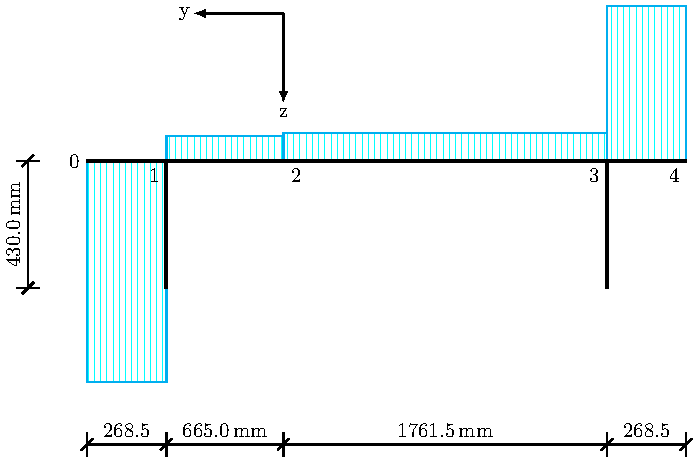
\includegraphics[width=0.7\textwidth]{img/diagram/mass/beam_diag_T.pdf}
\label{beam_diag_T}
\end{figure}

\begin{figure}[H]
\centering
\caption{\textbf{Bending moment} diagram due to the mass in motion.}
\vspace{0.1cm}
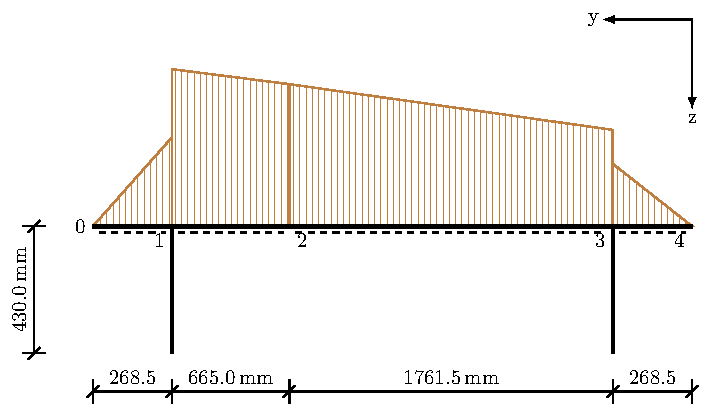
\includegraphics[width=0.7\textwidth]{img/diagram/mass/beam_diag_M.pdf}
\label{beam_diag_M}
\end{figure}


\section{Load Condition: Braking system}

When the train is moving at a certain velocity we need a force from the brake system to stop it in an opposite direction respect to the motion of the train.


\begin{figure}[H]
\centering     %%% not \center
\caption{Difference of the shape model between two different methods.}
\subfigure[]{\label{train_stop} \includegraphics[width=0.65\textwidth]{img/slides/train_stop.png}}
\subfigure[]{\label{train_stop_forces_position} \includegraphics[width=0.28\textwidth]{img/slides/train_stop_forces_position.png}}
\end{figure}

\begin{wrapfigure}{L}{7cm}
\includegraphics[height=0.32\textwidth]{img/slides/break_load_3D.png}
\caption{Axle scheme forces due to the breaking system}
\label{break_load_3D}
\end{wrapfigure}

The only way this force can come is from the journal, where the cabin is linked to the wheel-set. So we have two symmetric forces like drawn in figure \ref{train_stop_forces_position}. 
This braking forces than should come to the wheel from the friction with the railway.
To generate this braking force we need obviously a braking system. The brake characteristics are input of our problem:
\begin{flalign*}
\mu &= 0.35 & \text{(Brake friction coefficient)}\\
\text{F}_{\!f} &= 45000 \N & \text{(Maximum transversal force of the brake shoe)}
\end{flalign*}
So the maximum tangential force exerted by each brake is $\text{F}_f \cdot \mu = 15750 \N$


The break forces are directed upward like the masses in scheme \ref{beam_load_hinge} because this is the critical condition stated into the standard.
\\With a torque equilibrium around the axis we can obtain the break forces $\text{F}_{\!\text{FX}}$

\begin{equation}
2\, \mu \text{F}_f \, R_{b_1} + \mu \text{F}_f \, R_{b_2} = 2\, \text{F}_{\!\text{FX}} \, R
\end{equation}
%
Now we can get our unknown that is $\text{F}_{\!\text{FX}} = 15310 \N$

We must verify that we can withstand this force at the interface between wheel and rail. This is possible only if the force we must provide is less than the static friction limit that let to avoid slipping.

The limit is the normal force due to the weight on the wheel-set shared between the two wheels, times the friction coefficient:
\begin{equation}
\text{F}_{\!FX}^{limit} = 0.5\, \text{m} g \cdot \mu = 16677 \N
\end{equation}
Where the total mass on the wheel-set is $17000 \kg$ and the max friction between steel and steel is 0.2.
We have already evaluated $\text{F}_{\!FX}$ so we just need to compare it with the maximum possible. 
Since $\text{F}_{\!FX} = 15310 \N < 16677 \N = \text{F}_{\!FX}^{limit}$ the no slipping condition is verified.

To proceed calculating the internal forces diagram we need some other forces. 

The force scheme of the braking system are sketched in figure \ref{beam_load_break_yz}, figure \ref{beam_load_break_xy} and figure \ref{beam_load_break_torque}

\begin{figure}[H]
\centering
\caption{Loads on yz plane.}
\includegraphics[width=0.7\textwidth]{img/load/beam_load_break_yz.pdf}
\label{beam_load_break_yz}
\end{figure}


\begin{figure}[H]
\centering
\caption{Loads on xy plane.}
\includegraphics[width=0.7\textwidth]{img/load/beam_load_break_xy.pdf}
\label{beam_load_break_xy}
\end{figure}


\begin{figure}[H]
\centering
\caption{Torque on xy plane.}
\includegraphics[width=0.7\textwidth]{img/load/beam_load_break_torque.pdf}
\label{beam_load_break_torque}
\end{figure}

In xy plane, due to symmetry, it is straightforward to find the forces at the extremities of the axle. 
In the plane yz instead we need to apply two equilibrium  equation to find $\text{F}_{FZ_1}$ and $\text{F}_{FZ_2}$; with a momentum and vertical equilibrium equation we find that:
\begin{align}
\text{F}_{FZ_1} &= \frac{\mu \text{F}_f \cdot (3\, b - y_1 + s)}{2\, b} = 26341 \N \\
\text{F}_{FZ_1} &= \frac{\mu \text{F}_f \cdot (3\, b + y_1 + s)}{2\, b} = 20909 \N
\end{align}

Now we are able to compute the internal forces diagram of the system due to the braking system.

%%%%%%%%%%%%%%%%%%%%%%%%%%%%%%%%%%%%%%%%%%%%%%%%%%%%%%%%%%%%%%%%%%%%%%%%%%
%% xy plane
\begin{figure}[H]
\centering
\caption{\textbf{Shear} diagram due to the braking system in xy plane.}
\includegraphics[width=0.7\textwidth]{img/diagram/braking/beam_diag_break_xy_T.pdf}
\label{beam_diag_break_xy_T}
\end{figure}

\begin{figure}[H]
\centering
\caption{\textbf{Bending moment} diagram due to the braking system in xy plane.}
\includegraphics[width=0.7\textwidth]{img/diagram/braking/beam_diag_break_xy_M.pdf}
\label{beam_diag_break_xy_M}
\end{figure}

\begin{figure}[H]
\centering
\caption{\textbf{Torque} diagram due to the braking system in xy plane.}
\includegraphics[width=0.7\textwidth]{img/diagram/braking/beam_diag_break_torque.pdf}
\label{beam_diag_break_torque}
\end{figure}
%%%%%%%%%%%%%%%%%%%%%%%%%%%%%%%%%%%%%%%%%%%%%%%%%%%%%%%%%%%%%%%%%%%%%%%%%%%


%%%%%%%%%%%%%%%%%%%%%%%%%%%%%%%%%%%%%%%%%%%%%%%%%%%%%%%%%%%%%%%%%%%%%%%%%%
%% zy plane
\begin{figure}[H]
\centering
\caption{\textbf{Shear} diagram due to the braking system in yz plane.}
\includegraphics[width=0.7\textwidth]{img/diagram/braking/beam_diag_break_yz_T.pdf}
\label{beam_diag_break_xy_T}
\end{figure}

\begin{figure}[H]
\centering
\caption{\textbf{Bending moment} diagram due to the braking system in yz plane.}
\includegraphics[width=0.7\textwidth]{img/diagram/braking/beam_diag_break_yz_M.pdf}
\label{beam_diag_break_xy_M}
\end{figure}
%%%%%%%%%%%%%%%%%%%%%%%%%%%%%%%%%%%%%%%%%%%%%%%%%%%%%%%%%%%%%%%%%%%%%%%%%%%

We can sketch the whole diagram due to both mass in motion and breaking system in a 3D structure.


%%%%%%%%%%%%%%%%%%%%%%%%%%%%%%%%%%%%%%%%%%%%%%%%%%%%%%%%%%%%%%%%%%%%%%%%%%
%% 3D diagramm
\begin{figure}[H]
\centering
\caption{\textbf{Shear} diagram.}
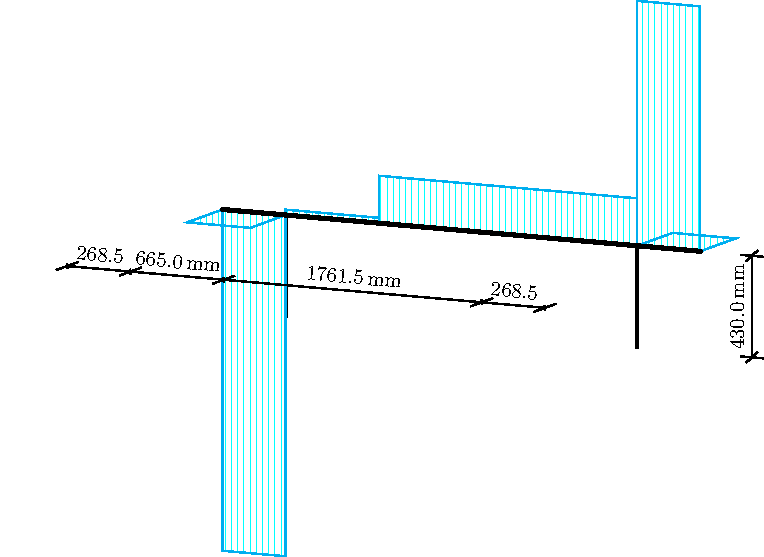
\includegraphics[width=0.7\textwidth]{img/diagram/beam_diag_tot_3D_T.pdf}
\label{beam_diag_tot_3D_T}
\end{figure}

\begin{figure}[H]
\centering
\caption{\textbf{Bending moment} diagram.}
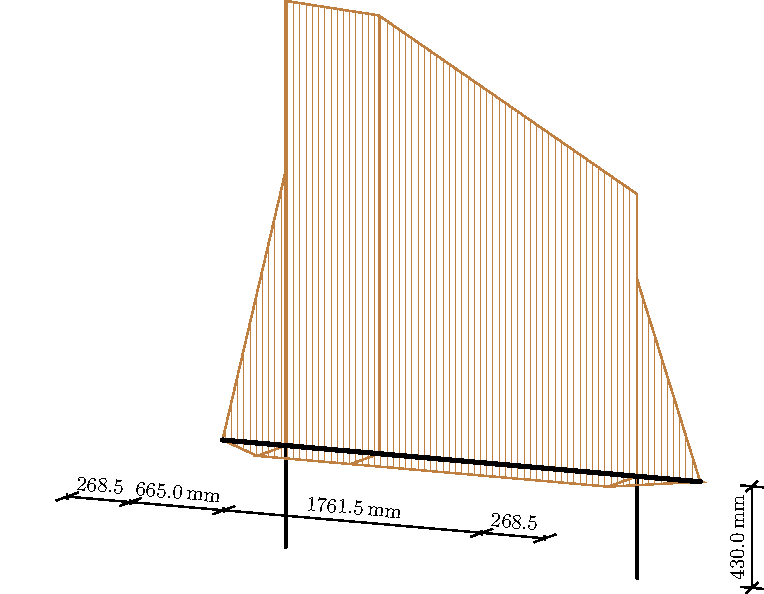
\includegraphics[width=0.7\textwidth]{img/diagram/beam_diag_tot_3D_M.pdf}
\label{beam_diag_tot_3D_M}
\end{figure}

\begin{figure}[H]
\centering
\caption{\textbf{Torque} diagram.}
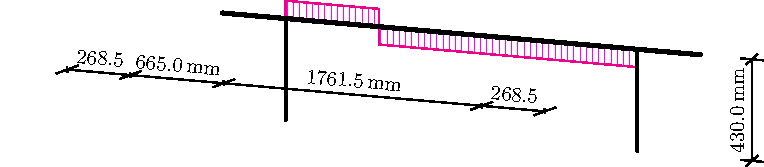
\includegraphics[width=0.7\textwidth]{img/diagram/beam_diag_tot_3D_torque.pdf}
\label{beam_diag_tot_3D_torque}
\end{figure}
%%%%%%%%%%%%%%%%%%%%%%%%%%%%%%%%%%%%%%%%%%%%%%%%%%%%%%%%%%%%%%%%%%%%%%%%%%%

The previous diagrams don't have the exact value of shear and moment and not all the graph are in scale one each other due to very different value so we collect all the numerical information in table \ref{table:no_brake} and \ref{table_break}.

\begin{table}[H]
\centering
\caption{Value of shear, bending moment and torque considering only mass in motion}
\label{table:no_brake}
\begin{tabular}{@{}l|ccc@{}}
\toprule
Point   & T                     & M                          & $M_{tot}$                  \\ \midrule
0 right & $\round{-112.376}\kN$ & $\round{0}\kNm$            & $\round{0}\kNm$            \\
1 left  & $\round{-112.376}\kN$ & $\round{30.172956}\kNm$    & $\round{30.172956}\kNm$    \\
1 right & $\round{12.773}\kN$   & $\round{53.17239309}\kNm$  & $\round{53.17239309}\kNm$  \\
2 left  & $\round{12.773}\kN$   & $\round{48.10789859}\kNm$  & $\round{48.10789859}\kNm$  \\
2 right & $\round{14.127}\kN$   & $\round{48.094945545}\kNm$ & $\round{48.094945545}\kNm$ \\
3 left  & $\round{14.118}\kN$   & $\round{32.614558545}\kNm$ & $\round{32.614558545}\kNm$ \\
3 right & $\round{78.64}\kN$    & $\round{21.11484}\kNm$     & $\round{21.11484}\kNm$     \\
4 left  & $\round{78.64}\kN$    & $\round{0}\kNm$            & $\round{0}\kNm$            \\ \bottomrule
\end{tabular}
\end{table}


\begin{table}[H]
\centering
\caption{Value of shear, bending moment and torque considering the braking system}
\label{table_break}
\begin{tabular}{@{}l|ccccccc@{}}
\toprule
Point   & T                   & M                       & $M_t$                 & T                    & M                       & $M_{tot}$                      & $M_{t_{tot}}$         \\ \midrule
0 right & $\round{15.31}\kN$  & $\round{0}\kNm$         & $\round{0}\kNm$       & $\round{-26.341}\kN$ & $\round{0}\kNm$         & $\round{0}\kNm$                & $\round{0}\kNm$       \\
1 left  & $\round{15.31}\kN$  & $\round{-4.110735}\kNm$ & $\round{0}\kNm$       & $\round{-26.341}\kN$ & $\round{7.0725585}\kNm$ & $\round{37.4716758713823}\kNm$ & $\round{0}\kNm$       \\
1 right & $\round{0}\kN$      & $\round{-4.110735}\kNm$ & $\round{2.1418}\kNm$  & $\round{-10.591}\kN$ & $\round{7.0725585}\kNm$ & $\round{60.3850340260041}\kNm$ & $\round{2.1418}\kNm$  \\
2 left  & $\round{0}\kN$      & $\round{-4.110735}\kNm$ & $\round{2.1418}\kNm$  & $\round{-10.591}\kN$ & $\round{11.27189}\kNm$  & $\round{59.521907187466}\kNm$  & $\round{2.1418}\kNm$  \\
2 right & $\round{0}\kN$      & $\round{-4.110735}\kNm$ & $\round{-2.1422}\kNm$ & $\round{5.159}\kN$   & $\round{11.27189}\kNm$  & $\round{59.5089850767705}\kNm$ & $\round{-2.1422}\kNm$ \\
3 left  & $\round{0}\kN$      & $\round{-4.110735}\kNm$ & $\round{-2.1422}\kNm$ & $\round{5.159}\kN$   & $\round{5.6150465}\kNm$ & $\round{38.4499784673141}\kNm$ & $\round{-2.1422}\kNm$ \\
3 right & $\round{-15.31}\kN$ & $\round{-4.110735}\kNm$ & $\round{-0.0004}\kNm$ & $\round{20.909}\kN$  & $\round{5.6140665}\kNm$ & $\round{27.0431615186902}\kNm$ & $\round{-0.0004}\kNm$ \\
4 left  & $\round{-15.31}\kN$ & $\round{0}\kNm$         & $\round{0}\kNm$       & $\round{20.909}\kN$  & $\round{0}\kNm$         & $\round{0}\kNm$                & $\round{0}\kNm$       \\ \bottomrule
\end{tabular}
\end{table}

\section{Section analysis}

The most critical section on the axle is that distant $110 \mm$ from the left wheel, immediately after the first brake in correspondence of the minimum diameter.

\begin{figure}[H]
\centering
\caption{Location of the critical section.}
\includegraphics[width=0.7\textwidth]{img/slides/critical_section.png}
\label{critical_section}
\end{figure}

We don't have the value of moments in that exact point but we can evaluate it with a linear interpolation. 
%
\begin{table}[H]
\centering
\begin{tabular}{@{}ccc@{}}
\toprule
N                      & M                         & $\text{M}_t$    \\ \midrule
$\round{53.487063}\kN$ & $\round{51.76736309}\kNm$ & $\round{0}\kNm$ \\ \bottomrule
\end{tabular}
\caption{Internal forces with mass in motion}
\end{table}
%
\begin{table}[H]
\centering
\begin{tabular}{@{}ccc@{}}
\toprule
N              & M                              & $\text{M}_t$         \\ \midrule
$\round{0}\kN$ & $\round{60.1455789131688}\kNm$ & $\round{2.1418}\kNm$ \\ \bottomrule
\end{tabular}
\caption{Internal forces with braking system}
\end{table}
%
Applying the beam theory we can get the stresses from the forces:

\begin{wrapfigure}[3]{l}{12cm}
\vspace{-0cm}
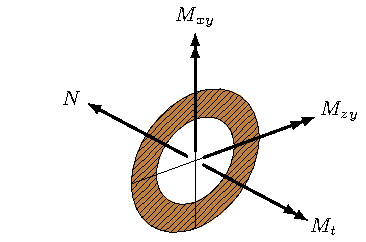
\includegraphics[width=0.4\textwidth]{img/beam_section.pdf}
\vspace{-0.0cm}
\caption{Scheme of forces and moment in the critical section}
\label{beam_section}
\end{wrapfigure}
%
%%%%%%%%%%%%%%%%%%%%%%%%%%%%%%%%%%%%%%%%%%%%%%%%%%%%%%%%%%%%%%%%%%%%%%%%%%%
%%%%%%%%%%%%%%%%%%%%%%%%%%%%%%%%%%%%%%%%%%%%%%%%%%%%%%%%%%%%%%%%%%%%%%%%%%%
%%%%%%%%%%%%%%%%%%    fondamentale    %%%%%%%%%%%%%%%%%%%%%%%%%%%%%%%%%%%%%
\leavevmode
%%%%%%%%%%%%%%%%%%%%%%%%%%%%%%%%%%%%%%%%%%%%%%%%%%%%%%%%%%%%%%%%%%%%%%%%%%%
%%%%%%%%%%%%%%%%%%%%%%%%%%%%%%%%%%%%%%%%%%%%%%%%%%%%%%%%%%%%%%%%%%%%%%%%%%%
%%%%%%%%%%%%%%%%%%%%%%%%%%%%%%%%%%%%%%%%%%%%%%%%%%%%%%%%%%%%%%%%%%%%%%%%%%%
%
\begin{flalign}
& \sigma_N = \frac{N}{A} &\\[0.5em]
& \sigma_M = \frac{M\cdot dist}{\text{J}_x} &\\[0.5em]
& \tau     = \frac{M_t\cdot dist}{\text{J}_p} &
\end{flalign}


~\\
\\
\\
\\
Before to proceed we must compute the geometrical properties of the section.
\begin{equation}
A = \pi \cdot (R^2 - r^2) = \round{22608} \mm^2
\end{equation}
\begin{equation}
\text{J}_x = \text{J}_y = \frac{\pi}{4} \cdot (R^4 - r^4) = \round{50868000} \mm^4
\end{equation}
\begin{equation}
\text{J}_p = \frac{\pi}{2} \cdot (R^4 - r^4) = 2\, \text{J}_x = \round{2*50868000} \mm^4
\end{equation}
\begin{conditions}
R & $90 \mm$;\\[0.5em]
r & $30 \mm$;
\end{conditions}

The stresses are maximum when the distance is the maximum possible so we set $dist = R = 90 \mm$ and finally in the two condition with or without brakes we can compute the stresses.

\begin{table}[H]
\centering
\begin{tabular}{@{}lccc@{}}
\toprule
         & $\sigma_N$                     & $\sigma_M$                     & $\tau$                         \\ \midrule
Braking system 	  & $\round{0}\MPa$                & $\round{106.414683144318}\MPa$ & $\round{1.89472753007785}\MPa$ \\
Mass in motion    & $\round{2.36584673566879}\MPa$ & $\round{91.5912298124558}\MPa$ & $\round{0}\MPa$                \\ \bottomrule
\end{tabular}
\caption{Stresses on the critical section}
\label{table:stresses_critical_section}
\end{table}

The section is in proximity of a change in diameter so we have to correct the values we have obtained multiplying that by the stress concentration factor $\text{K}_t$. We find the correct value in a proper diagram plotted in figure \ref{stress_concentration_factor} considering that in our case study:
\begin{flalign}
\frac{r}{d} &= \frac{15\mm}{180} = 1/12  = 0.0833&\\[0.5em]
\frac{D}{d} &= \frac{212\mm}{180\mm} = 53/45 = 1.1778&
\end{flalign}

\begin{figure}[H]
\centering
\caption{Stress concentration factor at the bottom of the transition between two cylindrical part.}
\includegraphics[width=0.7\textwidth]{img/slides/stress_concentration_factor.jpg}
\label{stress_concentration_factor}
\end{figure}

From figure \ref{stress_concentration_factor} we indentify that the stress concentration factor for our geometry is approximately 1.135; with this value we can obtain the final value for the stresses multiplying the previous results in table \ref{table:stresses_critical_section} by the stress concentration factor. Results are reported in table \ref{table:stresses_critical_section_final}.

\begin{table}[H]
\centering
\begin{tabular}{@{}lccc@{}}
\toprule
         & $\sigma_N$                     & $\sigma_M$                     & $\tau$                         \\ \midrule
Braking system 	  & $\round{1.135*0}\MPa$                & $\round{1.135*106.414683144318}\MPa$ & $\round{1.135*1.89472753007785}\MPa$ \\
Mass in motion    & $\round{1.135*2.36584673566879}\MPa$ & $\round{1.135*91.5912298124558}\MPa$ & $\round{1.135*0}\MPa$                \\ \bottomrule
\end{tabular}
\caption{Stresses on the critical section considering also the change in diameter. }
\label{table:stresses_critical_section_final}
\end{table}

\section{Shaft-Hub connection}

The connection between the shaft and the hub is obtained through a shrink fit. This means that the diameter of the hub is bigger than the diameter of the shaft, in this way, when they are connected there exists a compression force that keep the two different part together. The contact pressure strictly depends on the interference that is the difference between the two diameters.

We should:
\begin{itemize}
\item Determine the interference of the shrink fit which guarantees the transmission of the design torque.
		\begin{itemize}
			\item According with the design load, define the minimum interference $i_{\text{min}}$ which guarantees to transfer the load without slip.
			\item According to the standard (ISO), verify that with the defined drawing sizes, tolerances and roughness, the design interference $i_{\text{ISO}}$ is equal to, or larger than, $i_{\text{min}}$
		\end{itemize}
\item Verify that the proposed interference does not lead to a load which exceeds the strength of the material.
		\begin{itemize}
			\item Verify that, adopting $i_{\text{ISO}}$, the stress state does not lead to the failure of the components.
		\end{itemize}
\end{itemize}

We solve the problems applying many approaches. We start with the Analytical approach.

\subsection{Analytical Approach}

To apply the analytical approach is fundamental to define that let it to be valid and meaningful in the reality. The hypothesis are:
\begin{itemize}
\item We consider the nominal load with a service factor $K_s = 3$ so that $C_\text{lim} = K_s \cdot C_{\text{nominal}}$;
\item The hub is considered a disk with an hole;
\item The shaft is considered a disk with an hole;
\item The contact pressure on the contact surface is uniform.
\end{itemize}
The \emph{service factor} $K_s$ is taking into account impacts and irregular working conditions of the transmission. It is a safety coefficient and it increases the value of the design torque.

On the contact surface we have two components, one axial due to the reaction force $\text{Y}_1$ and one torsional due to the torque on the wheel.

\paragraph{Axial}

\begin{figure}[H]
\centering
%\caption{Beam loads.}
\includegraphics[width=0.7\textwidth]{img/load/beam_load.pdf}
\label{beam_load2}
\end{figure}

The value of $\text{Y}_1$ has already been calculated in equation \ref{force:Y1} and it is equal to $\round{53487} \N$.
This force acts as a shear stress in the contact surface. 
\begin{figure}[H]
\centering
%\caption{Beam loads.}
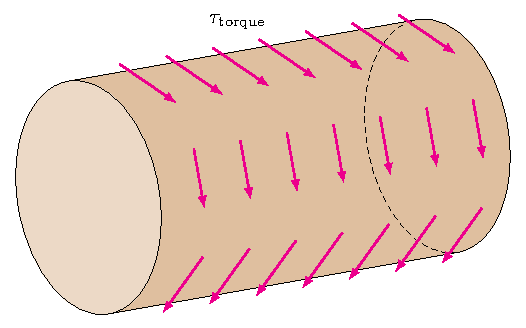
\includegraphics[width=0.5\textwidth]{img/cilinder_axial.pdf}
\label{cilinder_axial}
\end{figure}
%
The force is stress times surface so:
\begin{equation}
\text{Y}_1 = \tau \cdot A = \tau \cdot (\pi \, d \, L)
\end{equation}
%
The $\tau$ stress is the shear stress due to friction that prevent slipping and considering a friction coefficient $f = 0.2$, $\text{Y}_1$ results:
%
\begin{equation}
\text{Y}_1 = \tau_{\text{Y}} \cdot (\pi \, d \, L) = f\, p_{\text{Y}} \cdot \pi \, d \, L
\end{equation}
%
Since we are interested in the pressure we must revert the last equation to obtain $p_{\text{Y}}$. Moreover we must also consider the service factor $K_s$
\begin{equation}
p_{\text{Y}} = \frac{K_s \, \text{Y}_1}{f\, \pi \, d \, L} = \round{6.805820627723222} \MPa
\end{equation}

\paragraph{Torsional}
To calculate the nominal torque $\text{C}_n$ we must apply the moment balance on the left wheel.
\begin{figure}[H]
\centering
%\caption{Beam loads.}
\includegraphics[width=0.45\textwidth]{img/slides/break_load_3D.png}
\label{break_load_3D2}
\end{figure}
%
\begin{equation}
\text{C}_n = \text{F}_{FX}\cdot R - \mu \, \text{F}_f \cdot R_{b_1} = 2.15 \kNm
\end{equation}
%

Similarly to the axial case the torque is shear times surface times distance.
\begin{figure}[H]
\centering
%\caption{Beam loads.}
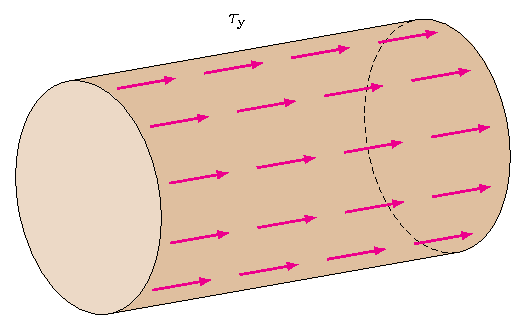
\includegraphics[width=0.5\textwidth]{img/cilinder_torque.pdf}
\label{cilinder_torque}
\end{figure}
%
\begin{equation}
\text{C}_n 
= \int_0^{2\pi} \tau \cdot dA \, \frac{d}{2}
= \int_0^{2\pi} \tau \cdot \left( L \, \frac{d}{2} \, d\alpha \right) \, \frac{d}{2} = \frac{1}{2} \, \tau \, L \, \pi \, d^2
\end{equation}
%
The $\tau$ stress is the shear stress due to friction that prevent slipping and considering a friction coefficient $f = 0.2$.
Since we are interested in the pressure we must revert the last equation to obtain $p_{\text{C}}$. 
Moreover we must also consider the service factor $K_s$. So the pressure $p_C$ results:
\begin{equation}
p_{\text{C}} = \frac{2 \, K_s \, \text{C}_n}{f\, \pi \, d^2 \, L} =  \round{2.580862418976949} \MPa
\end{equation}
%

The total pressure is not simply the sum of the two, since they are normal one to the other. So we must apply the Pythagorean theorem.
\begin{equation}
\label{eq:pressure}
p = \sqrt{p_\text{C}^2 + p_\text{Y}^2} = \round{7.278739261879797} \MPa
\end{equation}

From the geometry of the wheel(hub) and of the axle(shaft) and their tolerances we can calculate the maximum and the minimum interference.

\begin{table}[]
\centering
\caption{Dimension of wheel and axle with tolerances}
\label{table:wheel_axle_dimensions}
\begin{tabular}{@{}lccc@{}}
\toprule
\multicolumn{4}{c}{Wheel-Axle Assembly}                                    \\ \midrule
Component & Dimension          & Lower Limit         & Upper Limit         \\ \midrule
Wheel     & $\diameter$ 212 H7 & $\diameter 212.000$ & $\diameter 212.046$ \\
Axle      & $\diameter$ 212    & $\diameter 212.290$ & $\diameter 212.320$ \\ \bottomrule
\end{tabular}
\end{table}

From table \ref{table:wheel_axle_dimensions} we can evaluate the maximum and the minimum possible interference from drawings.
\begin{align}
i_\text{min} &= 212.290 - 212.046 = 0.244 \mm \\[0.5em]
i_\text{max} &= 212.320 - 212.000 = 0.320 \mm
\end{align}

We must verify that this designed interference is enough for withstanding the contact pressure.
To do that we apply the model of two hollowed cylinder both for the wheel and the axle. If the axle is quite similar to a cylinder the wheel instead has a complex shape.
We will apply two different modelling of the wheel, the former simply a hollowed cylinder, the latter a more redefined shape to which apply the Grammel's method 
The geometrical schematisation is sketched in figure \ref{fig:wheel_geometry}.

\begin{figure}[H]
\centering     %%% not \center
\caption{Difference of the shape model between two different methods.}
\subfigure[Simplified Schematization]{\label{fig:a}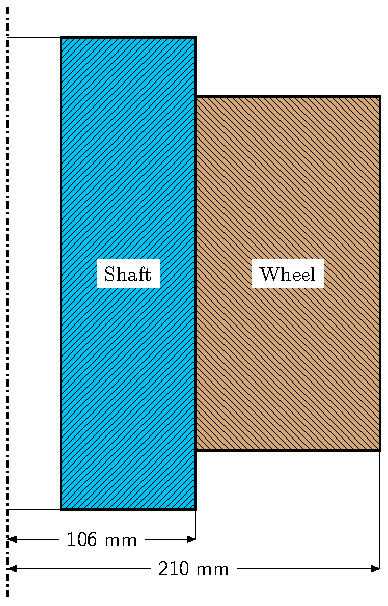
\includegraphics[height=0.4\textwidth]{img/wheel_geometry.pdf}}
\qquad
\qquad
\qquad
\subfigure[Grammel schematization]{\label{fig:b}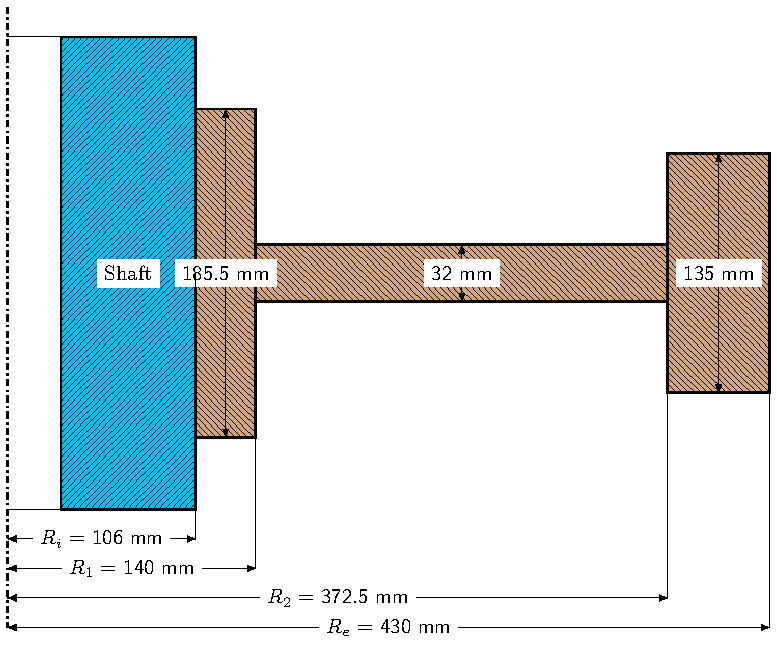
\includegraphics[height=0.4\textwidth]{img/wheel_geometry_grammel.pdf}}
\label{fig:wheel_geometry}
\end{figure}

We need two find a relationship between the interference and the pressure so that we can find if the interference designed is enough and from the maximum interference we can find the correspondent contact pressure.
The interference is the difference between the two diameter so:
\begin{equation}
\label{eq:interference}
i = d_\text{shaft} -d_\text{hub}
\end{equation}
When subjected to a certain pressure hole diameter in the hub expand and the shaft diameter shrink so and their final diameter must be the same.
\begin{equation}
\label{eq:diameters_equal}
d_\text{shaft} + \Delta d_\text{shaft} = d_\text{hub} + \Delta d_\text{hub}
\end{equation} 
The circumferential strain is $\varepsilon_\theta = \frac{u}{r}$ where $u$ is the radial displacement. 
\\The variation of the diameter is 2 times the radial displacement $u$ so:
\begin{equation}
\label{eq:delta_diameter}
\Delta d = 2\, u = 2\, r \cdot \varepsilon_\theta = d \, \varepsilon_\theta
\end{equation}
\begin{figure}[H]
\centering     %%% not \center
\caption{Pressure applied on wheel and axle.}
\subfigure[Hub (wheel)]{\label{fig:a}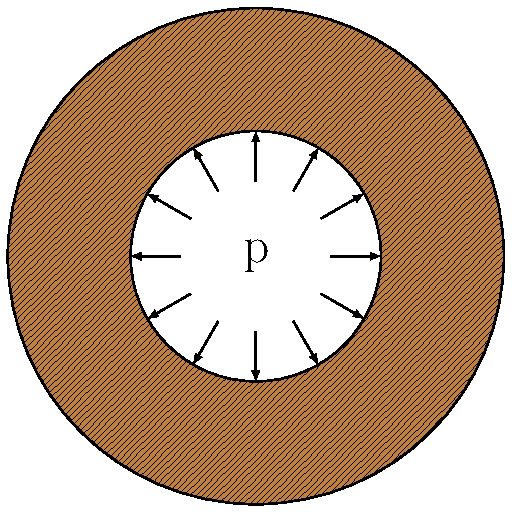
\includegraphics[height=0.4\textwidth]{img/hub_pressure.pdf}}
\qquad
\subfigure[Shaft (axle)]{\label{fig:b}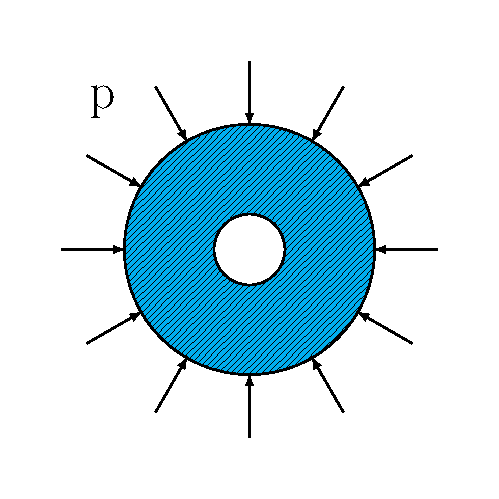
\includegraphics[height=0.4\textwidth]{img/shaft_pressure.pdf}}
\label{fig:shaft_hub_pressure}
\end{figure}
Applying this relationship both for the shaft and the hub we obtain:
\begin{align}
\Delta d_\text{shaft} &=  d_\text{shaft} \, \varepsilon_{\theta_\text{shaft}} =  d \, \varepsilon_{\theta_\text{shaft}} \\
\Delta d_\text{hub} &=  d_\text{hub} \, \varepsilon_{\theta_\text{hub}} =  d \, \varepsilon_{\theta_\text{hub}}
\end{align}
Since $d_\text{shaft} \approx d_\text{hub}$ we call $d \approx d_\text{shaft} \approx d_\text{hub}$
We calculate the strains, in particular the hoop one, based on the constitutive Hook's law.
\begin{align}
\varepsilon_{r} = \frac{1}{E}\, (\sigma_r - \nu \, \sigma_\theta)\\
\varepsilon_{\theta} = \frac{1}{E}\, (\sigma_\theta - \nu \, \sigma_r)
\end{align}
Applied for the shaft and the hub the circumferential strain are:
\begin{align}
\varepsilon_{\theta_\text{shaft}} = \frac{1}{E_\text{shaft}}\, (\sigma_{\theta_\text{shaft}} - \nu \, \sigma_{r_\text{shaft}}) \\[0.5em]
\varepsilon_{\theta_\text{hub}} = \frac{1}{E_\text{hub}}\, (\sigma_{\theta_\text{hub}} - \nu \, \sigma_{r_\text{hub}})
\end{align}
With the general equations of the stresses for the hollowed disk we can put in relationship the contact pressure with the radial and tangential stresses. 
The general solution is in the form:
\begin{align}
\begin{cases}{}
\sigma_r = A - \frac{B}{r^2} \\[0.5em]
\sigma_\theta = A + \frac{B}{r^2}
\end{cases}
\label{eq:hollow_cilinder_model_equation}
\end{align}
We have to apply the boundary conditions for the two cylinder.

\begin{wrapfigure}[5]{l}{6cm}
\vspace{-0cm}
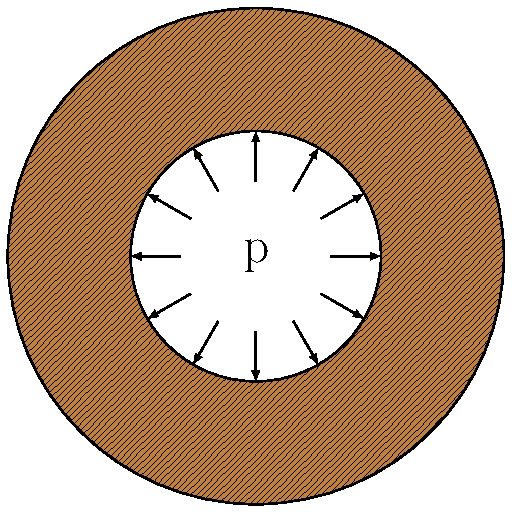
\includegraphics[height=0.3\textwidth]{img/hub_pressure.pdf}
\label{shaft_pressure}
\vspace{-0.0cm}
\end{wrapfigure}
\leavevmode
%
\begin{flalign}
&\sigma_r(r^i_\text{hub}) = -p &\\[0.5em]
&\sigma_r(r^e_\text{hub}) = 0 &
\end{flalign}
\begin{equation}
\label{eq:hub_stresses}
\begin{dcases}{}
\sigma_r(r) = \frac{p}{a^2-1} \left( 1 - \frac{(r^e_\text{hub})^2}{r^2} \right) \\[0.5em]
\sigma_\theta(r) = \frac{p}{a^2-1} \left( 1 + \frac{(r^e_\text{hub})^2}{r^2} \right) 
\end{dcases}
\end{equation}

\begin{wrapfigure}[4]{l}{6cm}
\vspace{-0cm}
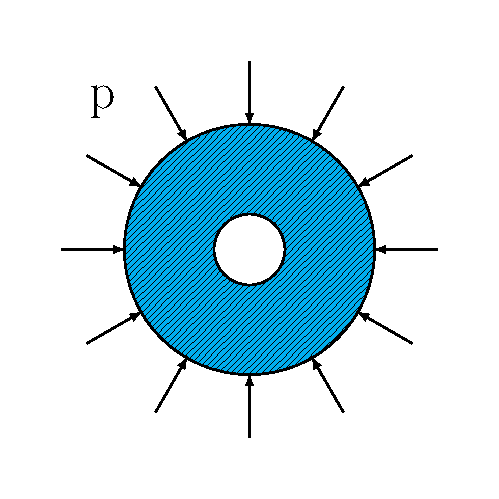
\includegraphics[height=0.3\textwidth]{img/shaft_pressure.pdf}
\label{shaft_pressure}
\vspace{-0.0cm}
\end{wrapfigure}
\leavevmode
%
\\
\begin{flalign}
&\sigma_r(r^i_\text{shaft}) = 0 &\\[0.5em]
&\sigma_r(r^e_\text{shaft}) = -p &
\end{flalign}
\begin{equation}
\label{eq:shaft_stresses}
\begin{dcases}{}
\sigma_r(r) = -\frac{p\cdot a^2}{a^2-1} \left( 1 - \frac{(r^i_\text{shaft})^2}{r^2} \right) \\[0.5em]
\sigma_\theta(r) = -\frac{p \cdot a^2}{a^2-1} \left( 1 + \frac{(r^i_\text{shaft})^2}{r^2} \right) 
\end{dcases}
\end{equation}

Now we are able to calculate the hoop strain for the two components in correspondence of the contact surface. The axle and the wheel are made by the same material.
\begin{align}
\label{eq:strain_shaft}
\varepsilon_{\theta_\text{shaft}} 
&= \frac{1}{E_\text{shaft}}\, (\sigma_{\theta_\text{shaft}} - \nu \, \sigma_{r_\text{shaft}}) 
= \frac{1}{E}\, \left(-p \, \frac{a_\text{s}^2+1}{a_\text{s}^2-1} - \nu \, (-p)\right) \\[0.5em]
\label{eq:strain_hub}
\varepsilon_{\theta_\text{hub}} 
&= \frac{1}{E_\text{hub}}\, (\sigma_{\theta_\text{hub}} - \nu \, \sigma_{r_\text{hub}}) 
= \frac{1}{E}\, \left(p \, \frac{a_\text{h}^2+1}{a_\text{h}^2-1} - \nu \, (-p)\right)
\end{align}

Finally we can express the interference as a function of the pressure combining together equations \ref{eq:interference}, \ref{eq:diameters_equal}, \ref{eq:delta_diameter}
with the two last equations \ref{eq:strain_shaft} and \ref{eq:strain_hub}. 
\begin{equation}
i = d_\text{shaft} -d_\text{hub} 
= \Delta d_\text{hub} - \Delta d_\text{shaft}
= d \, \left( \varepsilon_{\theta_\text{hub}} - \varepsilon_{\theta_\text{shaft}} \right)
= \frac{p\, d}{E} \cdot \left(\frac{a_\text{h}^2+1}{a_\text{h}^2-1} + \cancel{\nu}
+ \frac{a_\text{s}^2+1}{a_\text{s}^2-1} - \cancel{\nu} \right)
\end{equation}
\begin{equation}
\label{eq:interference and pressure}
i = \frac{p\, d}{E} \cdot \left(\frac{a_\text{h}^2+1}{a_\text{h}^2-1} + \frac{a_\text{s}^2+1}{a_\text{s}^2-1}\right)
\end{equation}
\begin{conditions}
a_\text{s} & $212 \mm / 60 \mm = \round{212/60}$;\\[0.5em]
a_\text{h} & $420 \mm / 212 \mm = \round{420/212}$;\\[0.5em]
\end{conditions}

For the pressure we have evaluated in equation \ref{eq:pressure} the interference $i = \round{0.022050303837754*1000} \E{-3} \mm$.
This is the minimum value of interference that generate a contact pressure sufficient to prevent the slipping through the connection. 
\\The value calculated is an elastic interference, to compare this value with the one designed previously we have to consider also the plastic deformation of the roughness on the surfaces.
\begin{equation}
i = i_\text{elastic} + 2 \, R_{P_\text{shaft}} + 2 \, R_{P_\text{hub}} 
\end{equation}
\begin{conditions}
R_{P_\text{shaft}} & $2 \, R_{a_\text{shaft}} = 2 \cdot 1.6 \E{-3} \mm = 3.2 \E{-3} \mm$;\\[0.5em]
R_{P_\text{hub}} & $2 \, R_{a_\text{hub}} = 2 \cdot 3.2 \E{-3} \mm = 6.4 \E{-3} \mm$;\\[0.5em]
\end{conditions}
So the final value of the interference results $i = \round{0.022050303837754*1000} \E{-3} \mm + 3.2 \E{-3} \mm + 6.4 \E{-3} \mm = \round{0.041250303837754*1000} \E{-3} \mm = 0.0413 \mm$ that is clearly less than the minimum interference chosen that is equal to $0.244 \mm$.

We can assert that for any diameter of the hub and of the shaft into the tolerances the slipping is prevented.

\paragraph{Maximum pressure}
The worst case for the contact pressure is when the interference is the maximum possible. 
Inverting equation \ref{eq:interference and pressure} the value of the pressure depending on the interference will be:
\begin{equation}
p = i \cdot \frac{E}{d} \cdot \left(\frac{a_\text{h}^2+1}{a_\text{h}^2-1} + \frac{a_\text{s}^2+1}{a_\text{s}^2-1}\right)^{-1}
\end{equation}
For the maximum value of $i = 0.320 \mm$ we have to find the value of the elastic interference:
\begin{equation}
i_\text{elastic} = i - 2 \, R_{P_\text{shaft}} - 2 \, R_{P_\text{hub}} = 0.320 \mm - 3.2 \E{-3} \mm + 6.4 \E{-3} \mm = 0.3008 \mm
\end{equation}
So the correspondent value of the pressure is $p_\text{max} = \round{99.293179181720730} \MPa$

With the pressure previously obtained, we are now able, through the model described by equations \ref{eq:hollow_cilinder_model_equation}, to find radial and circumferential stresses in the most stressed point for each body. 
The critical point is for the hub and for the shaft in the internal surface; the critical surface is not in both components where the pressure is applied.
We already have the expression for the stresses in any point for both the axle and the wheel from equations \ref{eq:hub_stresses} and \ref{eq:shaft_stresses}.
\begin{figure}[H]
\centering     %%% not \center
\caption{Pressure applied on wheel and axle.}
\subfigure[]{\includegraphics[width=0.45\textwidth]{img/hub_stresses.pdf}}
\qquad
\subfigure[]{\includegraphics[width=0.45\textwidth]{img/shaft_stresses.pdf}}
\label{fig:shaft_hub_stresses}
\end{figure}
Substituting the inner radius in the equations we get:
\\For the hub:
\begin{equation}
\label{eq:hub_stresses_value}
\begin{dcases}{}
\sigma_r(r_i) = \frac{p}{a^2-1} \left( 1 - \frac{(r^e_\text{hub})^2}{r_i^2} \right) = -p = \round{-99.293179181720730} \MPa\\[0.5em]
\sigma_\theta(r_i) = \frac{p}{a^2-1} \left( 1 + \frac{(r^e_\text{hub})^2}{r_i^2} \right) =  p \cdot\frac{a^2 + 1}{a^2-1} = \round{1.671886369035936e+02} \MPa
\end{dcases}
\end{equation}
\\And for the shaft:
\begin{equation}
\label{eq:shaft_stresses_value}
\begin{dcases}{}
\sigma_r(r_i) = -\frac{p\cdot a^2}{a^2-1} \left( 1 - \frac{(r^i_\text{shaft})^2}{r_i^2} \right) = \round{0} \MPa\\[0.5em]
\sigma_\theta(r_i) = -\frac{p \cdot a^2}{a^2-1} \left( 1 + \frac{(r^i_\text{shaft})^2}{r_i^2} \right) = -p \cdot\frac{2\,a^2}{a^2-1} = \round{-2.158781271837876e+02} \MPa
\end{dcases}
\end{equation}
From the value of the radial and circumferential stresses we can apply the Guest Tresca rule to find a summary value to stresses to compare with the yield strength of the material. The Guest Tresca stress is defined for ductile material as 
\begin{equation}
\sigma_\text{GT} = \abs{ \sigma_\text{max} - \sigma_\text{min} } \leq \frac{\sigma_\text{Y}}{\eta}
\end{equation}

To ensure not to have a static failure we can evaluate the safety factor of both component, and check if it is sufficiently greater than 1.
For the hub:
\begin{align}
\sigma_\text{GT} &= \abs{ \sigma_\text{max} - \sigma_\text{min} } = \round{1.671886369035936e+02} \MPa + \round{99.293179181720730} \MPa
= \round{1.671886369035936e+02 + 99.293179181720730} \MPa \\
\eta &= \frac{\sigma_\text{Y}}{\sigma_\text{GT}} = \frac{545}{\round{1.671886369035936e+02 + 99.293179181720730}} 
= \round{545/(1.671886369035936e+02 + 99.293179181720730)} \gg 1
\end{align}
For the shaft:
\begin{align}
\sigma_\text{GT} &= \abs{ \sigma_\text{max} - \sigma_\text{min} } = \round{0} \MPa + \round{2.158781271837876e+02} \MPa
= \round{2.158781271837876e+02} \MPa \\
\eta &= \frac{\sigma_\text{Y}}{\sigma_\text{GT}} = \frac{545}{\round{2.158781271837876e+02}} 
= \round{545/(2.158781271837876e+02)} \gg 1
\end{align}
Both the wheel and the axle are safety for what that concern the static assessment due to the shrink-fit pressure in every possible condition of interference in the range of the tolerances.


\subsection{Fem Analysis}

To perform a more realistic analysis we model the shrink fit connection adopting axis-symmetric finite elements. To do that we have to respect the hypotheses that both the \emph{\textbf{load}} and the \emph{\textbf{geometry}} must be axis-symmetric. In this case this two fundamental hypotheses are valid so our model is meaningful.

\begin{figure}[H]
\centering     %%% not \center
\caption{Shape model for the fem analysis of the axle and the wheel.}
\subfigure[Axle]{\includegraphics[height=0.4\textwidth]{img/slides/shaft_fem.png}}
\qquad
\qquad
\qquad
\subfigure[Wheel]{\includegraphics[height=0.4\textwidth]{img/slides/hub_fem.png}}
\label{wheel_geometry_fem}
\end{figure}

The stress configuration resultant is represented in figure \ref{fig:stresses_fem}.

\begin{figure}[H]
\centering
\caption{Von Mises stresses from the fem analysis.}
\includegraphics[width=0.8\textwidth]{img/slides/stresses_fem.png}
\label{fig:stresses_fem}
\end{figure}

From this analysis we are mainly interested in the contact pressure onto the surface between the hub and the shaft. So it is useful to plot how this pressure changes along the contact path. This result is drawn in figure \ref{fig:conctact_pressure_fem}.

\begin{figure}[H]
\centering
\caption{Contact pressure along the path.}
\includegraphics[width=0.8\textwidth]{img/contact_pressure_fem.pdf}
\label{fig:conctact_pressure_fem}
\end{figure}

Is interesting to notice that differently from the previous hypothesis we have made of contact pressure, in reality this is just a simplification. In fact the pressure tends to increase near the boundaries. This behaviour is interesting because in the analytical model we have considered only the part of the shaft in contact with the wheel; but in reality the shaft continues even after the wheel, and this part tries to prevent the other to deform. In this way near the boundaries we have a sort of constraint from the remaining part of the axle that increases the pressure. 
Apart from that the previous result of $ \round{99.293179181720730} \MPa$ is quite good as a mean value along the path.













\newpage
\section{The Grammel Method}
Previously we have studied the shaft-hub connection considering the shaft as a simple hollowed cylinder with the same mass and inertia of the real shape. This kind of schematisation is quite rough. We can improve the results dividing the shape in more than one sub-cylinder and than applying the Grammel's method to obtain a more refined contact mean pressure. 
This method works dividing the shape in simpler section and the evaluate the internal pressures between them. It follows the principle of the force method; the iperstatic unknowns are the pressures, and we get them applying the compatibility equation.

The wheel is modelled as drawn in figure \ref{wheel_geometry_grammel}.

\begin{figure}[H]
\centering     %%% not \center
\caption{Difference of the shape model between two different methods.}
\subfigure[Grammel schematization]{\label{fig:a}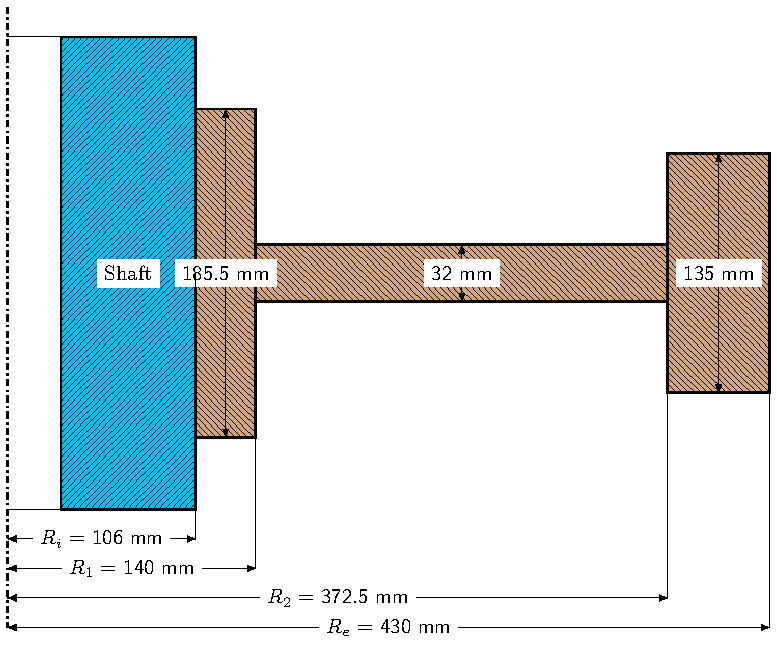
\includegraphics[height=0.4\textwidth]{img/wheel_geometry_grammel.pdf}}
\qquad
\qquad
\qquad
\subfigure[Previous schematization]{\label{fig:b}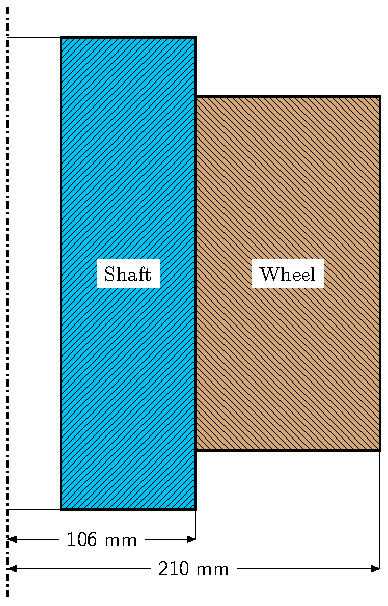
\includegraphics[height=0.4\textwidth]{img/wheel_geometry.pdf}}
\label{wheel_geometry_grammel}
\end{figure}

%\begin{figure}[H]
%\centering
%\caption{Modellization for Grammel's Method.}
%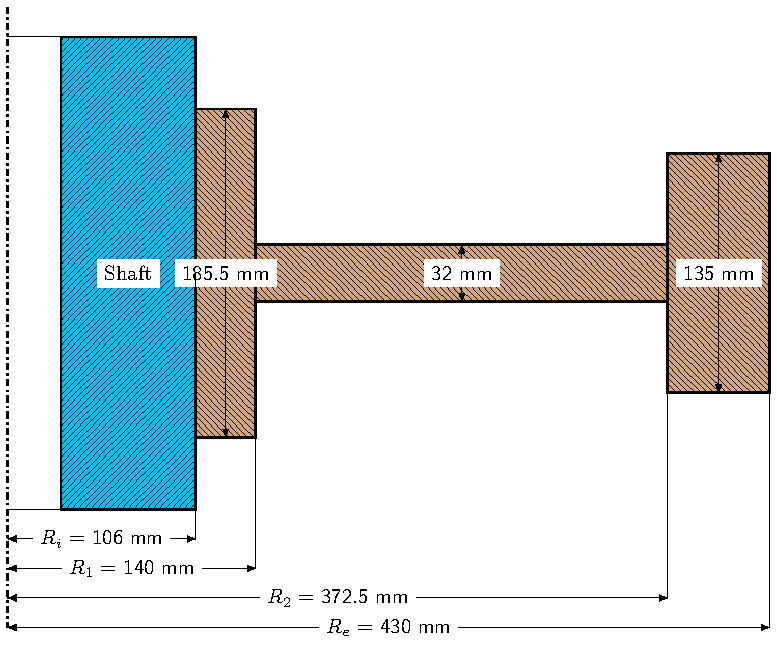
\includegraphics[width=0.5\textwidth]{img/wheel_geometry_grammel.pdf}
%\label{wheel_geometry_grammel}
%\end{figure}

\begin{wrapfigure}{R}{4cm}
\vspace{-0.0cm}
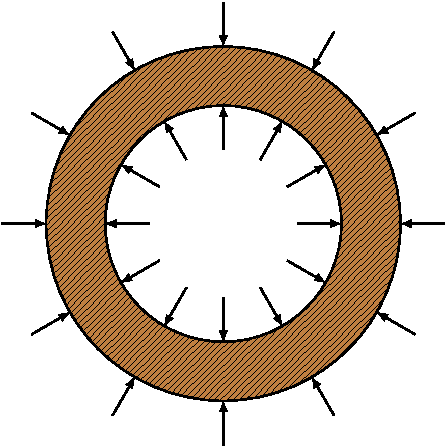
\includegraphics[width=0.2\textwidth]{img/pressure.pdf}
\end{wrapfigure}

We have now 3 different hollowed cylinder in which apply the axisymmetric model; in each part we can write the radial stress and the tangential stress along the radius as:

\begin{equation}
\begin{cases}{}
\sigma_r = A_i + \frac{B_i}{r^2} \\ 
\sigma_{\theta} = A_i - \frac{B_i}{r^2} \\ 
\end{cases}
\label{sigma_r_theta} 
\end{equation}

In this case with 3 section we have 6 unknown coefficients so we must find 6 compatibility conditions.
We can start applying the boundaries condition at the internal radius $R_i$ and at the external radius $R_e$.

\[\begin{cases}{}
\sigma_{R_1}(r_i) = -p \\ 
\sigma_{R_3}(r_e) = 0 \\ 
\end{cases}\]

Moreover we have to guarantee the radial equilibrium and the circumferential compatibility at the interface between section 1 and 2 and between section 2 and 3. Summarizing in total we have 4 more equation:

\[\begin{cases}{}
\sigma_{R_1}(r_1)\cdot h_1 = \sigma_{R_2}(r_1)\cdot h_2  \\ 
\sigma_{R_2}(r_2)\cdot h_2 = \sigma_{R_3}(r_2)\cdot h_3  \\ 
\end{cases}\]

Where $h_1$ and $h_2$ are the height of the hollowed cylinders.

\begin{equation}
[\begin{cases}{}
\sigma_{\theta_1}(r_1)-\nu\sigma_{R_1}(r_1) = \sigma_{\theta_2}(r_1)-\nu\sigma_{R_2}(r_1) \\ 
\sigma_{\theta_2}(r_2)-\nu\sigma_{R_2}(r_2) = \sigma_{\theta_3}(r_2)-\nu\sigma_{R_3}(r_2) \\ 
\end{cases}
\end{equation}

Substituting into each stress the equations \ref{sigma_r_theta} we have 6 unknowns in 6 equation. We can write the linear system in matrix form as follow in matrix \ref{matrix_expanded}.

\begingroup
\renewcommand*{\arraystretch}{2}
\begin{equation}
\label{matrix_expanded}
\begin{bmatrix}
1     & \dfrac{1}{r_i^2}      & 0        & 0                    & 0        & 0                   \\
0     & 0                    & 0        & 0                    & 1        & \dfrac{1}{r_e^2}     \\
h_1   & \dfrac{h_i}{r_1^2}    & -h_2     & -\dfrac{h_2}{r_1^2}   & 0        & 0                   \\
0     & 0                    & h_2      & \dfrac{h_2}{r_2^2}    & -h_3     & -\dfrac{h_3}{r_2^2}  \\
1-\nu & -\dfrac{1+\nu}{r_1^2} & -(1-\nu) & \dfrac{1+\nu}{r_1^2}  & 0        & 0                   \\
0     & 0                    & 1-\nu    & -\dfrac{1+\nu}{r_2^2} & -(1-\nu) & \dfrac{1+\nu}{r_2^2}
\end{bmatrix}
\cdot
\begin{bmatrix}
A\\ B\\ C\\ D\\ E\\ F
\end{bmatrix}
=
\begin{bmatrix}
-p\\ 0\\ 0\\ 0\\ 0\\ 0
\end{bmatrix}
\end{equation}
\endgroup
%
Or in a more compact way as $[M]\underline{x}=\underline{b}$. The solution in obtained simply solving the linear system: $\underline{x}=[M]^{-1}\cdot\underline{b}$. The solution we get is function of the internal pressure $p$ that is an unknown of our problem:

\begin{equation}
\underline{x} 
=
\begin{bmatrix}
A\\ B\\ C\\ D\\ E\\ F
\end{bmatrix}
=
\begin{bmatrix}
0.7823\\ -20026\\ 0.0358\\ -27905\\ 0.1178\\ -21781
\end{bmatrix}
\cdot p
\end{equation}

Now we must apply the same procedure as before to find the relationship between the contact pressure $p$ and the interference $i$.

\begin{equation}
\label{iel_iso}
i_{el} = i^{\text{max}}_{\text{ISO}} - i_{\text{pl}} = 0.320 - 0.0192 = 0.301\,\text{mm}
\end{equation}
But the elastic interference is also the difference between the diameter of the hub (wheel) and the shaft.
\begin{equation}
i_{el} = d_{\text{shaft}} - d_{\text{hub}} = \Delta d_h - \Delta d_s
\end{equation}
As we have seen before, substituting equation \ref{sigma_r_theta} for the two components, the interference can be written as
\begin{equation}
\label{iel_p}
i_{el} = \frac{p \cdot d}{E} \cdot \left( \frac{a_h^2+1}{a_h^2-1} + \frac{a_s^2+1}{a_s^2-1} \right)
\end{equation}

Combining together equations \ref{iel_iso} and \ref{iel_p} we obtain the final value of the contact pressure that values 75.9 MPa.

Finally we can compare in figure \ref{fig:contact_pressure_total} the three different solutions:
\begin{itemize}
\item Finite element analysis;
\item Simplified shape;
\item Grammel's method.
\end{itemize}

\begin{figure}[H]
\centering
\caption{Contact pressure along the path in the three cases.}
\includegraphics[width=0.8\textwidth]{img/contact_pressure_total.pdf}
\label{fig:contact_pressure_total}
\end{figure}


\section{Fatigue Analysis}

In order to perform the fatigue assessment on the railway axle we need to retrieve some data:
\begin{itemize}
\item Understand the theory of fatigue design;
\item The properties of the material and the geometry of the components;
\item Evaluation of $\text{K}_t$;
\item Description of the finite element model;
\item Calculation of the loads for the fatigue analysis.
\end{itemize}
%
In particular we can apply two different criterion:
\begin{itemize}
\item The \textbf{global} approach bases on the analytical nominal stress;
\item The \textbf{local} approach bases on the numerical local stresses;
\end{itemize}

We have to deal with multi-axial fatigue loads that can be split into two components, one mean and one alternated. The criterion the let us to manage such complexity is the \textbf{Sines criterion}. It states that:
\begin{equation}
\sigma_{AR} = \dfrac{\sigma^\star}{1-\dfrac{\text{I}_m}{\text{UTS}}} < \dfrac{\sigma'_e}{\eta}
\label{eq:sigma_AR}
\end{equation}
\begin{conditions}
\sigma^\star & Sines equivalent stress;\\[0.5em]
\text{I}_m & first stress invariant;\\[0.5em]
\text{UTS} & ultimate tensile strength;\\[0.5em]
\sigma'_e & endurance limit of the mechanical component;\\[0.5em]
\eta & safety factor;\\[0.5em]
\end{conditions}
We can express the previous quantities as function of material and geometrical properties and mean and alternated stresses. In fact:\\
The Sines equivalent stress only considers the alternated component of the stresses and is equal to:
\begin{equation}
\sigma^\star = \sqrt{\text{S}_{x_a}^2 + \text{S}_{y_a}^2 + \text{S}_{z_a}^2
- \text{S}_{x_a} \, \text{S}_{y_a} - \text{S}_{x_a} \, \text{S}_{z_a} - \text{S}_{y_a} \, \text{S}_{z_a}
+ 3\, \tau_{xy_a}^2 + 3\, \tau_{xz_a}^2 + 3\, \tau_{yz_a}^2 }
\end{equation}
The first invariant stress instead is only taking into account the mean stress and it is defined as the sum of the principal mean stresses.
\begin{equation}
\text{I}_m = \text{S}_{x_m} + \text{S}_{y_m} + \text{S}_{z_m}
\end{equation}
The endurance limit instead depends mainly on the material resistance but it can be reduces a lot when the component is really different from the standard specimen in term of dimensions ($\text{m}_d$), surface finishing ($\text{m}_s$) and presence of notch ($\text{k}_f$)
\begin{equation}
\sigma'_e = \dfrac{0.4\, \text{UTS} \, \text{m}_s \, \text{m}_d}{\text{k}_f}
\label{eq:sigma_e_prime}
\end{equation}
Is interesting to notice that usually, in presence of bending moment, $\sigma_e$ is equal to $0.5\, \text{UTS}$ but in this case is instead just $0.4\, \text{UTS}$. The standard in fact expects to be safety side, but suggest to impose the dimensional coefficient $\text{m}_d$ equal to 1.  $\text{k}_f$ is also provided by the standard and it is set to 1.2.

Since we have the model of the axle we can perform a finite element analysis to get the fatigue stress concentration factor.
At this point we can apply different approaches:
\begin{itemize}
\item Global method
\begin{itemize}
\item Analytical (Previously done with figure \ref{stress_concentration_factor});
\item Numerical;
\end{itemize}
\item Local method.
\end{itemize}

The main difference between local and global methods is that in the global we take the most stressed point, and there comparing the real stress with the theoretical one, we obtain the stress concentration factor $\text{k}_t$ in that point, instead, with the local method we directly use the value of the real stress from the simulation and with that we evaluate the safety factor in any point; then we simply take the minimum safety factor on the piece. The local approach down not take into account $\text{k}_t$.

\subsection{Global method - Numerical}

The model of the axle is created thanks to the 3D part module and than, after we have set the properties of the material, the loads are applied;
Reference points are created on the two points of connection with the wheels and on the connection with the wheel-set in order to better place the forces acting on the component and the boundaries conditions (i.e bearings ). The points and their surfaces are coupled with a kinematic bound that is needed to be sure that all the fitting surfaces will be rigidly moved when a load in applied on the reference points.

Consider the load case when brake forces are NOT activated:
\begin{itemize}
\item Only coach weight and lateral forces are considered;
\item The load is composed by a main bending component plus a minor axial force.
\end{itemize}

But the coefficient $\text{k}_t$ depends on the geometry and on the applied load and due to this we have to evaluate two of it:
\begin{itemize}
\item for bending load;
\item for axial load.
\end{itemize}
From now on, we only consider bending loads, due to their major effects on global stresses.

After the application of the forces we can run the simulation and create a new reference system that has its origin in the correspondence of the maximum value of the stress.

The actual considered forces are highlighted in figure \ref{fig:fatigue_loads}.

\begin{figure}[H]
\centering
\caption{Forces and moments applied on the axle.}
\includegraphics[width=0.5\textwidth]{img/slides/fatigue_loads.png}
\label{fig:fatigue_loads}
\end{figure}

We mesh the model (figure \ref{fig:fatigue_mesh}) and we apply the analysis for all the different load conditions in which we are interested in:
\begin{itemize}
\item Mean forces without brakes;
\item Alternated forces without brakes;
\item Mean forces with brakes;
\item Alternated forces with brakes;
\end{itemize}

\begin{figure}[H]
\centering
\caption{Mesh of the railway axle.}
\includegraphics[width=0.8\textwidth]{img/fatigue/fig1.png}
\label{fig:fatigue_mesh}
\end{figure}

Once we have find the more stressed point is important to attach to that point the correct frame to get the principal stresses in the right directions.


\begin{figure}[H]
\centering     %%% not \center
\caption{Strains with solid finite elements and model without ports.}
\subfigure[Alternated component with only the weight]{\includegraphics[height=0.3\textwidth]{img/fatigue/weight_alternated/fig1.png}}
\subfigure[Alternated component also with brakes]{\includegraphics[height=0.3\textwidth]{img/fatigue/brakes_alternated/fig1.png}}
\label{fig:solidmodel3_strain_bottom_ports}
\end{figure}

Firstly we need the nominal value and then we must take the results from the finite element analysis. The nominal values are reported in table \ref{table:stresses_critical_section} and for sake of simplicity are copied in table \ref{table:stresses_critical_section_copy}.

\begin{table}[H]
\centering
\begin{tabular}{@{}lccc@{}}
\toprule
         & $\sigma_N$                     & $\sigma_M$                     & $\tau$                         \\ \midrule
Braking system 	  & $\round{0}\MPa$                & $\round{106.414683144318}\MPa$ & $\round{1.89472753007785}\MPa$ \\
Mass in motion    & $\round{2.36584673566879}\MPa$ & $\round{91.5912298124558}\MPa$ & $\round{0}\MPa$                \\ \bottomrule
\end{tabular}
\caption{Nominal stresses on the critical section}
\label{table:stresses_critical_section_copy}
\end{table}

Instead the results of the maximum stresses from Abaqus are:

\begin{table}[H]
\centering
\begin{tabular}{@{}lcc@{}}
\toprule
           			& $\sigma_x^\text{alternated}$ & $\text{I}_m$     \\ \midrule
Braking system 	    & $\round{126.7650}\MPa$ 	   & $\round{-1.5845}\MPa$				\\
Mass in motion      & $\round{109.1630}\MPa$	   & $\round{-1.5825}\MPa$				\\ \bottomrule
\end{tabular}
\caption{Maximum numerical stresses}
\label{table:stresses_critical_section_abq}
\end{table}

So we can now evaluate the stress concentration factor for the two cases. The calculations are reported in the following equations.
\\For the case \textbf{without} the braking system:
\begin{equation}
\text{K}_t = \frac{\sigma_\text{max}}{\sigma_\text{nominal}} = \frac{\round{109.1630}\MPa}{\round{91.5912298124558}\MPa} = 
\round{109.1630 / 91.5912298124558}
\end{equation}
For the case \textbf{with} the braking system:
\begin{equation}
\text{K}_t = \frac{\sigma_\text{max}}{\sigma_\text{nominal}} = \frac{\round{126.7650}\MPa}{\round{106.414683144318}\MPa} = 
\round{126.7650 / 106.414683144318}
\end{equation}
As we can see we get the same result for both the two cases.

The stress concentration factor is required for evaluating the \emph{fatigue} stress concentration factor. This parameter is always smaller the the static case and it can be calculated as:
\begin{equation}
\text{K}_f = 1 + q \, (\text{K}_t - 1)
\end{equation}
\begin{conditions}
q & notch sensitivity;\\[0.5em]
\end{conditions}
The parameter $q$ can be obtained from the Neuber formula that states:
\begin{equation}
q = \dfrac{1}{ 1 + \sqrt{ \dfrac{\rho}{r}  }}
\label{eq:neuber_formula}
\end{equation}
\begin{conditions}
\rho & is the curvature;\\[0.5em]
r    & is the radius of the notch.\\[0.5em]
\end{conditions}
The curvature $\rho$ depends on the material ultimate tensile strength; for the steel S355 $\sqrt{\rho}$ is approximately 0.3, as we can obtain from plot \ref{fig:curvature}.

\begin{figure}[H]
\centering
\caption{Curvature function of $\text{R}_m$}
\includegraphics[width=0.8\textwidth]{img/slides/curvature.png}
\label{fig:curvature}
\end{figure}
%
Substituting everything into equation \ref{eq:neuber_formula} we obtain:
\begin{equation}
q = \dfrac{1}{ 1 + \sqrt{ \dfrac{\rho}{r}  }}
= \round{0.928108986997839}
\label{eq:neuber_formula_value}
\end{equation}
%
Finally we obtain $\text{K}_f$ that is $\text{K}_f = 1 + q \, (\text{K}_t - 1) = \round{1 + 0.928108986997839 * (1.19 - 1)}$.
%
From equation \ref{eq:sigma_e_prime} we obtain the endurance limit specifically of the axle component.
\begin{equation}
\sigma'_e = \dfrac{0.4\, \text{UTS} \, \text{m}_s \, \text{m}_d}{\text{k}_f}
 = \dfrac{200 \MPa}{ 1.18}
= \round{ 200 / 1.18 } \MPa
\label{eq:sigma_e_prime_value}
\end{equation}

To perform the global assessment finally we need the alternated and mean stress tensor as stated in equation \ref{eq:sigma_AR}; We have to evaluate it in both the two load conditions considering only the theoretical stresses since the stress concentration factor has already taken into account in $\sigma'_e$.
\\For the case \textbf{without} the braking system:
\begin{equation}
\sigma_\text{alternated} = 
\begin{bmatrix}
    0 & 0 & 0 \\
    0 & \round{91.591} & 0 \\
    0 & 0 & 0 \\
\end{bmatrix}
\qquad
\qquad
\sigma_\text{mean} = 
\begin{bmatrix}
    0 & 0 & 0 \\
    0 & \round{2.3658} & 0  \\
    0 & 0 & 0 \\
\end{bmatrix}
\end{equation}
So the alternated reversed equivalent $\sigma_\text{AR}$ results:
\begin{equation}
\sigma_\text{AR} = \dfrac{\sigma^\star}{1-\dfrac{\text{I}_m}{\text{UTS}}}
= \dfrac{\round{91.591} \MPa}{1 - \dfrac{2.3658 \MPa}{600 \MPa}}
= \round{91.591 / (1 - 2.3658 / 600)} \MPa
\end{equation}
And the safety factor is:
\begin{equation}
\eta = \dfrac{\sigma'_e }{\sigma_\text{AR}} = \dfrac{\round{200 / 1.18 }}{91.95} = \round{200 / 1.18 / 91.95} > 1.5
\end{equation}
%
For the case \textbf{with} the braking system:
\begin{equation}
\sigma_\text{alternated} = 
\begin{bmatrix}
    0 & 0 & 0  \\
    0 & \round{106.4147} & 0  \\
    0 & 0 & 0  \\
\end{bmatrix}
\qquad
\qquad
\sigma_\text{mean} = 
\begin{bmatrix}
    0 & \round{-1.895} & 0  \\
    \round{-1.895} & \round{2.3658} & 0  \\
    0 & 0 & 0 \\
\end{bmatrix}
\end{equation}
So the alternated reversed equivalent $\sigma_\text{AR}$ results:
\begin{equation}
\sigma_\text{AR} = \dfrac{\sigma^\star}{1-\dfrac{\text{I}_m}{\text{UTS}}}
= \dfrac{\round{106.4147} \MPa}{1 - \dfrac{2.3658 \MPa}{600 \MPa}}
= \round{106.4147 / (1 - 2.3658 / 600)} \MPa
\end{equation}
And the safety factor is:
\begin{equation}
\eta = \dfrac{\sigma'_e }{\sigma_\text{AR}} = \dfrac{\round{200 / 1.18 }}{106.84} = \round{200 / 1.18 / 106.84} > 1.5
\end{equation}
%







\subsection{Local method}

The main point that has to be clearly stated is that in this approach the fatigue notch effect coefficient should not have evaluated and considered into the formulas since it is already present in the values of the stresses obtained from the Abaqus simulations.

Into the Sines formula we have the effects of the alternated stresses separated from the one of the mean stresses; Due to this we have to perform four simulations:
\begin{itemize}
\item Mean forces without brakes;
\item Alternated forces without brakes;
\item Mean forces with brakes;
\item Alternated forces with brakes;
\end{itemize}

\paragraph*{Mean forces without brakes\\}
In case of the model without brakes the only mean forces are due to the axial forces. The stresses generated, as we know, are small compared to that related to bending.

\begin{figure}[H]
\centering
\caption{Mean forces due to weight}
\includegraphics[width=0.7\textwidth]{img/slides/mean_weight_load.png}
\end{figure}

\paragraph*{Alternated forces without brakes\\}
Instead the alternate stresses are due to the other forces that generate bending or due to moments their self.

\begin{figure}[H]
\centering
\caption{Alternated forces due to weight}
\includegraphics[width=0.7\textwidth]{img/slides/alt_weight_load.png}
\end{figure}
%%%%%%%%%%%%%%%%%%%%%%%%%%%%%%%%%%%
\paragraph*{Mean forces with brakes\\}
The load that contributes to the medium load are:
\begin{itemize}
\item Moments around Y axis produce constant torsion effects;
\item Axial forces (in Y direction) produce constant axial effects.
\end{itemize}

\begin{figure}[H]
\centering
\caption{Mean forces due to weight}
\includegraphics[width=0.7\textwidth]{img/slides/mean_brakes_load.png}
\end{figure}

\paragraph*{Alternated forces with brakes\\}
All the loads (except those producing torsion and axial forces) induce alternate stress components.

\begin{figure}[H]
\centering
\caption{Alternated forces due to weight}
\includegraphics[width=0.7\textwidth]{img/slides/alt_brakes_load.png}
\end{figure}

From the two simulations of the alternated stresses we need to extract the \textbf{Von Mises} stress, instead from the two simulations of the mean stresses we need the \textbf{first invariant $\text{I}_m$ }. Abaqus can return the so-called pressure that is defined as the opposite of a third of the first invariant, so $\text{I}_m = - 3 \, \text{pressure}$.\\
The results are plotted in figure \ref{fig:comparison_stresses}

\begin{figure}[H]
\centering
\caption{Comparison of stresses component in various cases.}
\includegraphics[height=0.4\textwidth]{img/comparison_stresses.pdf}
\label{fig:comparison_stresses}
\end{figure}

With the stresses previously calculated now we are able to evaluate the alternated reversed equivalent stress for any point along the most stresses section of the axle.

\begin{equation}
\sigma_\text{AR} = \dfrac{\sigma^\star}{1-\dfrac{\text{I}_m}{\text{UTS}}}
\end{equation}
%
\begin{conditions}
\sigma^\star & Von Mises stress;\\[0.5em]
\text{I}_m & the sum of $\text{I}_m$ due to the external load and due  to the shrink fit;\\[0.5em]
\end{conditions}
%
Finally the safety factor is:
\begin{equation}
\eta = \frac{\sigma_\text{e'}}{\sigma_\text{AR}}
\end{equation}
Where the fatigue limit of the component is provided from the standard and it is equal to $200 \MPa$. 

\begin{figure}[H]
\centering
\caption{Comparison of local safety factor with and without brakes.}
\includegraphics[height=0.4\textwidth]{img/comparison_eta.pdf}
\label{fig:comparison_eta}
\end{figure}

As we can imagine the critical condition is in presence of both the weight and the brakes. The minimum of the safety factor in the worst case equals to $\round{1.6695}$.

\end{document}

